\documentclass[tikz,border=2pt]{standalone}
\usepackage{amsmath}
\usepackage{pgfplots}
\pgfplotsset{compat=1.18}
\usetikzlibrary{arrows.meta}
\begin{document}
% Offered work for arrivals at 1,4,5,8,9,12 (lambda = 1/2): staircases with jumps 1.5 (rho = 0.75)
% and 2.5 (rho = 1.25) against the capacity line t of one server; at t = 12: 9 and 15 versus 12.
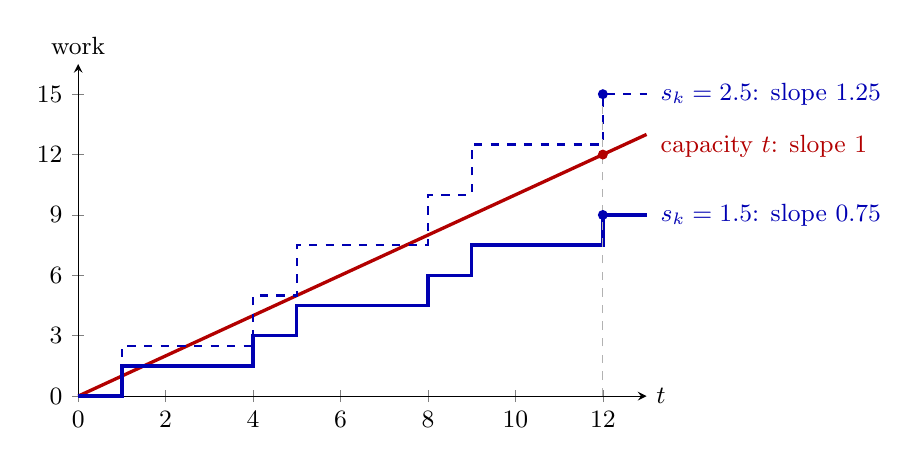
\begin{tikzpicture}[font=\small, >={Latex[length=2mm]}]
  \begin{axis}[
    axis lines=left, xmin=0, xmax=13, ymin=0, ymax=16.5,
    xtick={0,2,4,6,8,10,12}, ytick={0,3,6,9,12,15},
    xlabel={$t$}, ylabel={work},
    xlabel style={at={(axis description cs:1,0)}, anchor=west},
    ylabel style={rotate=-90, at={(axis description cs:0,1)}, anchor=south},
    width=8.8cm, height=5.8cm, clip=false
    ]
    \addplot[red!70!black, very thick, domain=0:13, samples=2] {x};
    \addplot[blue!70!black, very thick, const plot]
      coordinates {(0,0) (1,1.5) (4,3) (5,4.5) (8,6) (9,7.5) (12,9) (13,9)};
    \addplot[blue!70!black, thick, dashed, const plot]
      coordinates {(0,0) (1,2.5) (4,5) (5,7.5) (8,10) (9,12.5) (12,15) (13,15)};
    \draw[gray!60, thin, dashed] (axis cs:12,0) -- (axis cs:12,15);
    \fill[blue!70!black] (axis cs:12,9) circle (1.8pt);
    \fill[blue!70!black] (axis cs:12,15) circle (1.8pt);
    \fill[red!70!black] (axis cs:12,12) circle (1.8pt);
    \node[blue!70!black, anchor=west] at (axis cs:13.1,15) {$s_k=2.5$: slope $1.25$};
    \node[red!70!black, anchor=west] at (axis cs:13.1,12.4) {capacity $t$: slope $1$};
    \node[blue!70!black, anchor=west] at (axis cs:13.1,9) {$s_k=1.5$: slope $0.75$};
  \end{axis}
\end{tikzpicture}
\end{document}
